%!TEX root = ../doc.tex
\chapter{ROS: Setup und Tools}\label{sec:rosSetup}
Damit mit ROS und ROS-I gearbeitet werden kann müssen zuerst einige Installationen und Setups vorgenommen werden. Diese werden in diesem Abschnitt erläutert. Gleichzeitig werden einige ROS spezifische Tools erläutert, die das Arbeiten und auch Debuggen erleichtern können.
\section{Auswahl Distribution}
Für die Implementierung des Basis ROS-Systems, sowie für ROS-Industrial musste eine geeignete ROS-Distribution (siehe Abschnitt \ref{sec:Distro}) gewählt werden. Die Wahl viel Dabei auf die Distribution ROS Kinetic Kame. Diese Distribution wurde gewählt, da sie im Vergleich zu ihrer Vorgängerversion (ROS Jade Turtle) einige Verbesserungen mit sich bringt. Gleichzeitig ist es von Vorteil, dass die Distribution schon ca. ein Jahr im Einsatz ist und somit ein Grossteil der verfügbaren Packages von ROS schon auf die Version Kinetic porträtiert wurden.

\section{Auswahl IDE}
Grundsätzlich kann Sourcecode in ROS, wie jede andere Software auch, mit einem Texteditor und einem passenden Compiler generiert werden. Für ROS stehen eine Vielzahl an \glspl{IDE} zur Verfügung. Aufgrund von bereits vorhandener Erfahrung wurde Visual Studio Code verwendet, welches mit einem Plugin erweitert werden kann um CMakeFiles und auch ROS spezifische Files besser zu unterstützen. 

\section{Installation}
Die Installation von ROS und ROS-I können in Ubuntu über \gls{apt} installiert werden. Eine detaillierte Installationsanleitung ist auf dem ROS-Wiki\footnote{ROS: \url{http://wiki.ros.org/kinetic/Installation}\\ROS-I:\url{http://wiki.ros.org/Industrial/Install}} zu finden. Hier wird nur auf die wichtigsten Details eingegangen, da die Installationsanleitung eher umfangreich ist. Wichtig bei der Installation ist, das für ROS und ROS-Industrial die selben Distributionen installiert werden, zudem ist es zu empfehlen alle ROS und ROS-I Packages zu installieren. Dies verhindert spätere Komplikationen durch nicht vorhandene Packages. Nach der Installation von ROS sollten direkt die Abhängigkeiten von ROS initialisiert (\mintinline{bash}{rosdep init}) und upgedatet (\mintinline{bash}{rosdep update}) werden.\\
\newpage
\section{Workspace}
Nach der Installation muss ein Workspace eingerichtet werden welcher für Catkin konform ist. Dies über die \gls{IDE} möglich, geht aber am einfachsten über folgende Konsolenbefehle:
\begin{code}
	\begin{minted}{bash}
$ source /opt/ros/kinetic/setup.bash	# Source ROS setupscript
$ mkdir -p ~/catkin_ws/src				# erstellen benötigter Ordner	
$ cd ~/catkin_ws/
$ catkin_make							# compilieren
$ source devel/setup.bash				# Source Workspace setupscript
	\end{minted}
	\vspace{-15pt}
	\caption{Konsolenbefehle zur Generierung eines Catkin-Workspace}
	\label{code:catkinWS}
\end{code}
Im Workspace sollten sich nun die Unterordner build und devel befinden, gleichzeitig sollte sich im Ordner src die Datei CMakelists.txt befinden.
Das Setupscript eines Workspaces muss beim starten eines neuen Terminals immer neu eingelesen werden, es bietet sich an diese Zeile im File \verb|~/.basrc| hinzuzufügen, damit dies nicht mehr notwendig ist. 

\section{Nützlichetools}
In ROS gibt es eine Vielzahl nützlicher Konsolenbefehle und Tools hier eine kurze Auflistung der in dieser Arbeit meist gebrauchten.

\subsection{rqt}
Bei rqt handelt es sich um ein sehr mächtiges Tool in ROS, welches es ermöglicht auf fast alle Datenströme (messages, topics, services) zuzugreifen und diese zu visualisieren. Das Standartmenü kann über die Konsole mit dem Befehl \mintinline{bash}{rqt} gestartet werden, dazu muss jedoch bereits ein ROS-Master aktiv sein. Mithilfe diverser Plugins können weitere nützliche Funktionen von rqt genutzt werden. Eine der Hilfreichsten ist dabei rqt\_graph welche mit dem gleichlautenden Konsolenbefehl gestartet werden kann. Mit rqt\_graph können alle aktiven Nodes und die auf den Topics publizierten Nachrichten visualisiert werden. Somit kann schnell und einfach überprüft werden, ob ein Node läuft und ob Topics vorhanden sind. 
\begin{figure}[h!]
	\centering
	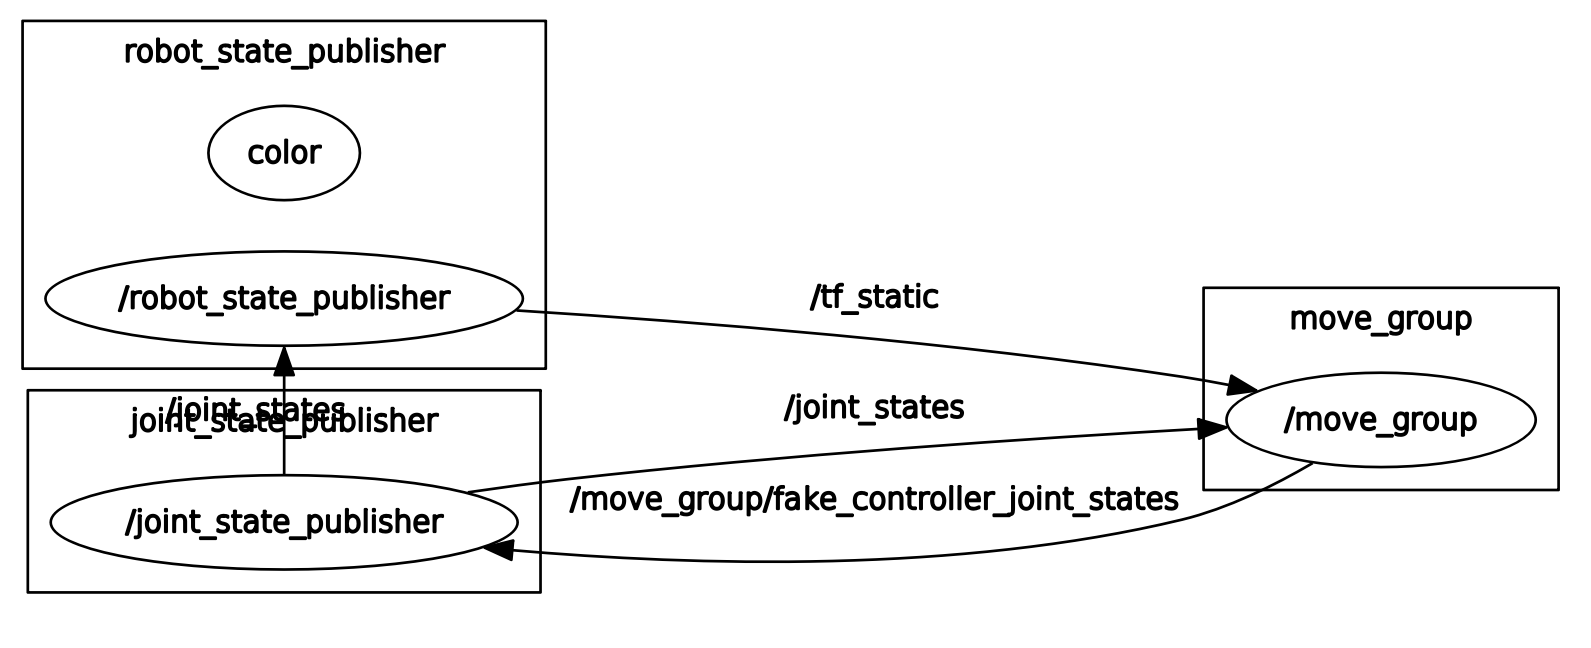
\includegraphics[width=0.8\textwidth]{rqtGraph}
	\caption{Ausgabe von rqt\_graph}
	\label{fig:rqtGraph}
\end{figure}

\subsection{Node}
\begin{description}[align=left]
	\item[rosnode list] Gibt eine Liste aller laufenden Nodes aus
	\item[rosnode info nodename] Gibt Informationen über einen laufenden Node aus
	\item[rosnode ping nodename] Pingt einen laufenden Node
	\item[rosnode kill nodename] Beendet einen laufenden Node
\end{description}

\subsection{Topics}
\begin{description}[align=left]
	\item[rostopic list] Gibt eine Liste mit allen registrierten Topics aus
	\item[rostopic echo /topicname] Gibt alle auf dem Topic publizierten Nachrichten aus
	\item[rostopic hz /topicname] Gibt die Frequenz an mit der Publiziert wird
	\item[rostopic pub /topicname data] Publiziert auf einem Topic die mitgegebenen Daten
\end{description}

\subsection{Parameterserver}
\begin{description}
	\item[rosparam list] Gibt eine Liste aller gespeicherten Parameternamen aus
	\item[rosparam get /paramname] Gibt den gespeicherten Variabelwert zurück
	\item[rosparam set /paramname] Über-/schreibt einen neuen Wert auf den Parameterserver
	\item[rosparam delete /paramname] Löscht den angegebenen Parameter vom Server
\end{description}

